\section{Evaluation}
\label{sec:eval}

\subsection{Experiment setups}
We deployed ZooKeeper service and the CRAQamo server nodes on Princeton University's $tux.cs.princeton.edu$ virtual machines.
These machines have 4 Intel(R) Xeon(R) CPUs which each run at 3.07GHz. The nodes were configured to listen on local network ports for our testing to be both easier and more consistent. To simulate the high communication latency that might occur when servers are geopraphically separated or operating under bad network environment, we used ``ncat'' in port forwarding mode to receive request connections on a different network port, then relay the data with a controlled delay to the actual listening port of CRAQamo servers. The delay is inserted in a per data line fashion which differs from the per-packet latency that exists in real TCP/IP networks. In our setting the amount of delay in $x$ miliseconds will
translate to $2x$ milisecond of round trip time, or RTT in real long range network communications. 

We used a chain size of 3 nodes for the tests, and the eventually consistent requests are replied when 2 servers respond (including the one handling the request). A client program that generates requests at a fixed rate is used to test the latency of CRAQamo's operations. 

\subsection{Effects of network delay on request latency}
\vspace{-5mm}
\begin{figure}[hbt]
\centering
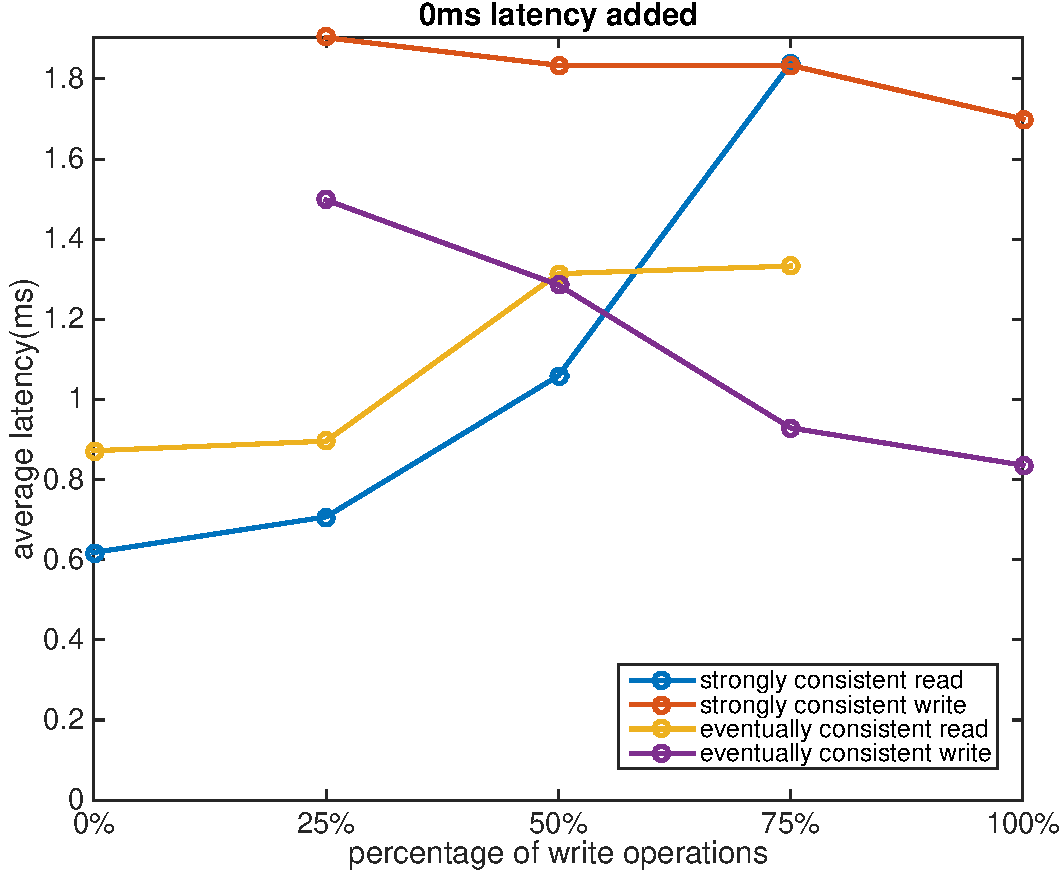
\includegraphics[width=\linewidth]{figures/latency_0.pdf}
\caption{with no network delay}
\label{fig:latency_0}
\end{figure}

\begin{figure}[hbt]
\centering
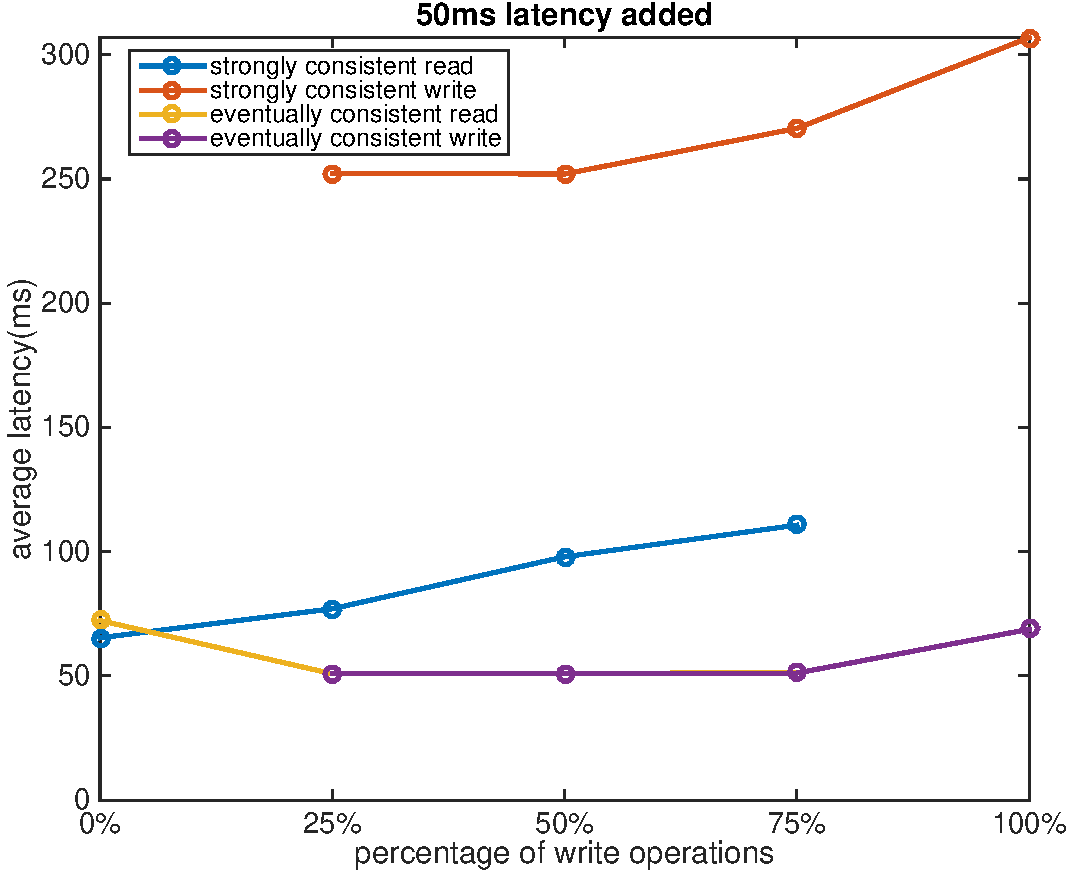
\includegraphics[width=\linewidth]{figures/latency_50.pdf}
\caption{with 50ms network delay}
\label{fig:latency_50}
\end{figure}

\begin{figure}[hbt]
\centering
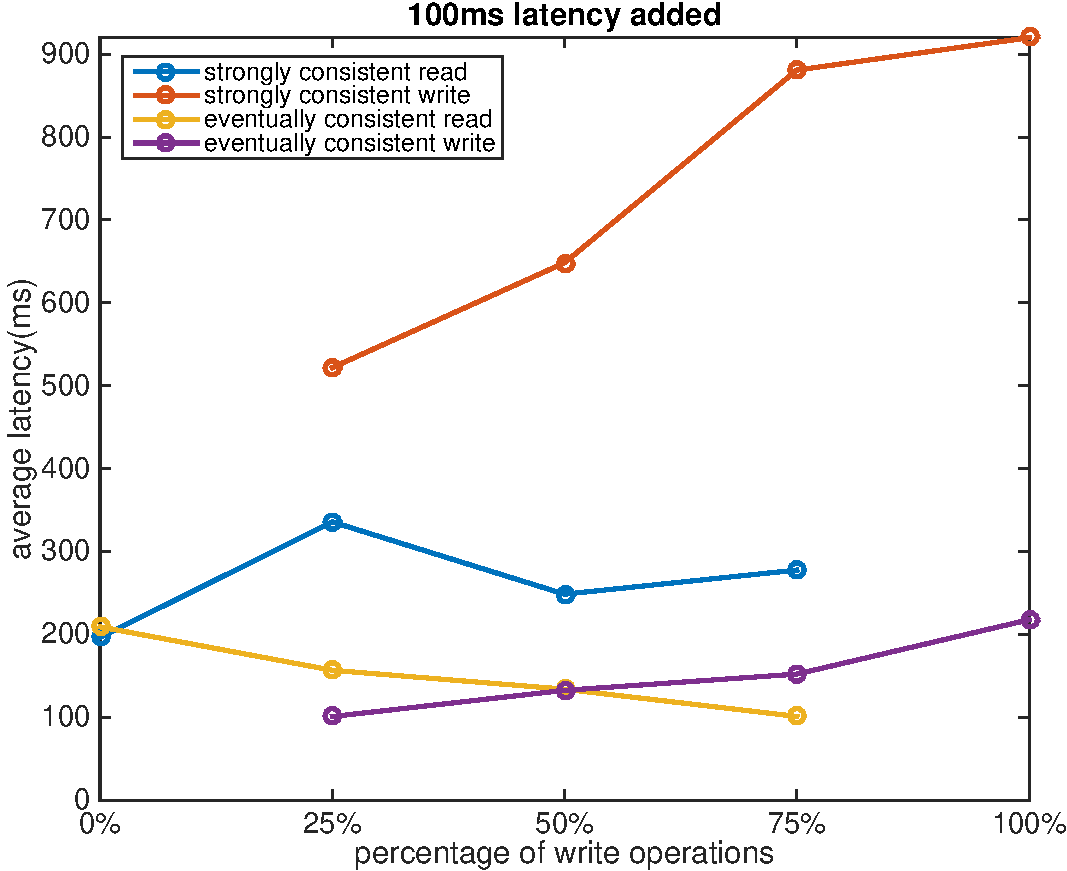
\includegraphics[width=\linewidth]{figures/latency_100.pdf}
\caption{with 100ms network delay}
\label{fig:latency_100}
\end{figure}
\vspace{-2mm}


CRAQamo was tested using 3 different network delay amounts of 0ms, 50ms and 100ms. We also varied the proportion of write requests to better illustrate CRAQamo's ability to support faster writes in eventual consistency model. We recorded the average latency of the four types of requests, namely strongly consistent read (SC read), strongly consistent write (SC write), eventually consistent read (EC read), and eventually consistent write (EC write). SC operations are the ones supported by the original CRAQ. Note that SC and EC operations are not mixed togather for this section of evaluation, therefore SC reads are only executed together with SC writes while EC reads are only executed together with EC writes. 

Under perfect network conditions , EC reads are slightly slower than SC reads when write operations are not dominant (see Figure \ref{fig:latency_0}), because EC reads needs multiple servers to agree on a value before replying back to the client while in most cases in SC mode, the servers know that their copy of the data is the most recent committed, this is one of CRAQ's selling point. As there are more writes SC reads get slower than EC read because writes must propagate in the chain. EC writes are consistently faster than SC writes under different write proportions due to the fact that EC writes does not need to go from chain head to chain tail sequencially.

With 50ms of network delay (100ms RTT), latency of EC operations differentiate from SC operations  (see Figure \ref{fig:latency_50}). EC reads can take almost 50\% less time than SC reads when there are more write requests, while EC writes are close to 5 times faster than SC writes on average. The gain comes from sacrificing consistency.

When network delay is more significant at 100ms (200ms RTT), typical for a long distance network connection, EC operations really show their advantage in latency  (see Figure \ref{fig:latency_100}). Latency of EC reads and writes stay in the range of 100ms to 200ms, for different write proportions, while SC operations become intolerably irresponsive (e.g., SC write at almost 900ms with 75\% writes).

\subsection{Effect of mixing different consistency models}
\vspace{-2mm}
\begin{figure}[h]
\centering
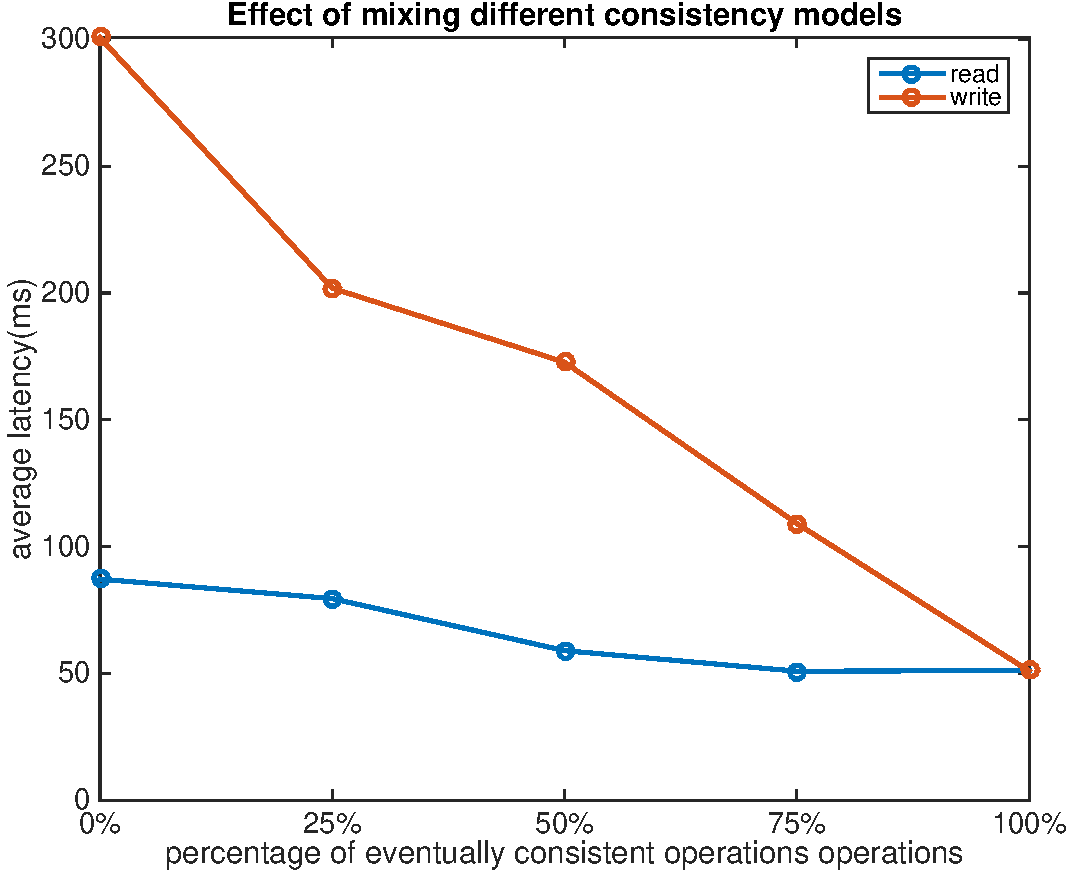
\includegraphics[width=\linewidth]{figures/mix.pdf}
\caption{mixing SC/EC operations}
\label{fig:mix}
\end{figure}
\vspace{-5mm}

To analyse the effect on latency of mixing SC/EC operations, we tested CRAQamo with varying proportions of EC/SC operations at 50\% writes and 50ms delay using the same setup from the previous section. The average latency of read and write operations (including both SC and EC) is shown in Figure \ref{fig:mix}.  As there are more EC operations inflight, the average latency dropped fast monotonically. Indeed EC operations can be executed much faster and are suitable for non-sensitive data.


